
Code capabilities of \llms{} are evaluated and compared using natural language to code generation tasks.
However, this only captures one dimension of code-related capabilities.
% Indeed, real-world software engineering requires expertise in tasks beyond just \textit{generation}, such as synthesizing informative test cases, debugging incorrect code, understanding existing code, and writing documentation.
% These tasks are not just additional bookkeeping; they are crucial parts of the software development process and contribute to improving the quality, maintainability, and reliability of the code~\citep{10.1145/1134285.1134288}.
% This also applies to \llms{} and adopting similar workflows can enable the models to perform better code generation.
AlphaCodium~\citep{ridnik2024code} developed an intricate \llm{} pipeline for solving competition coding problems. 
By combining natural language reasoning, test case generation, code generation, and self-repair, they achieve significant improvements over a naive direct code generation baseline, showcasing the importance of these broader capabilities.
Motivated by this, we propose a holistic evaluation of \llms{} using a suite of evaluation setups that capture a broader range of code-related capabilities.

\noindent Specifically, we evaluate code \llms{} in four scenarios, namely code generation, self-repair, code execution, and test output prediction.
Our selection criterion was to pick settings that are useful components in code \llm{} workflows 
and in addition, have clear and automated evaluation metrics.

\noindent Following we describe each of these scenarios in detail.

\begin{figure*}[!tb]
    \centering
    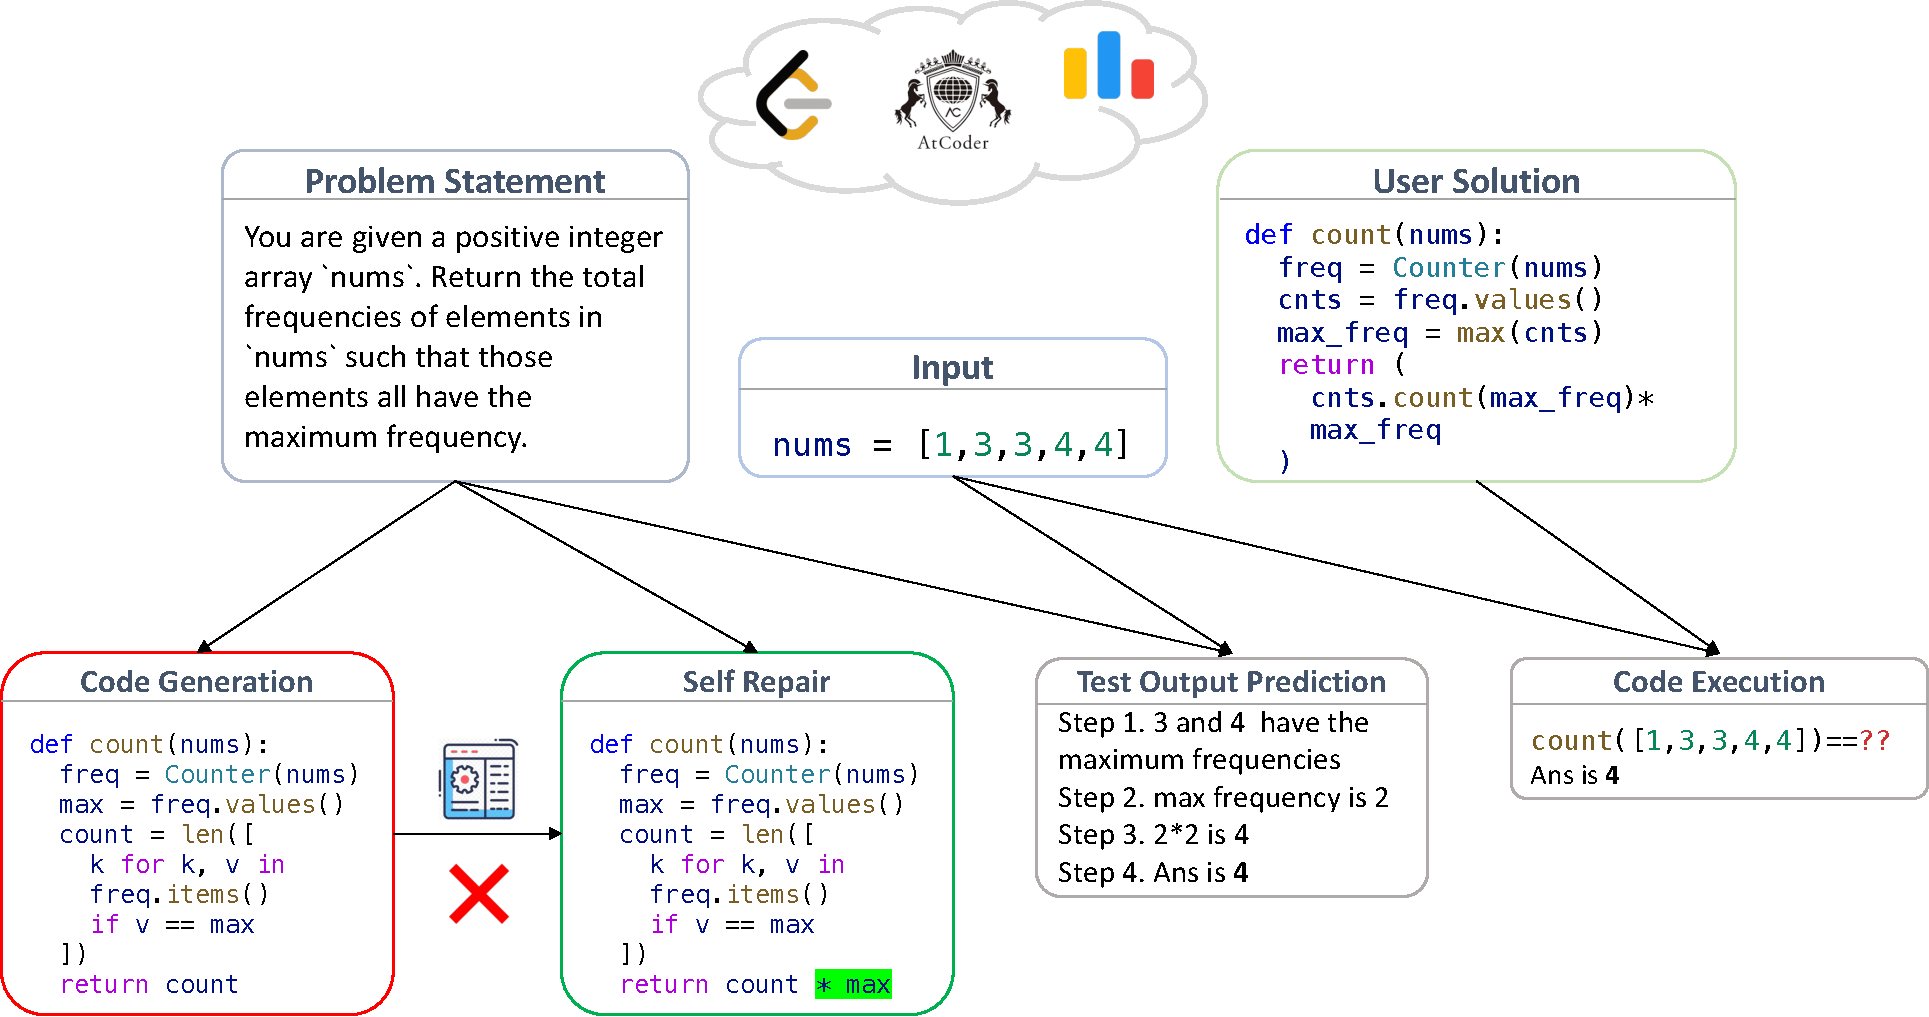
\includegraphics[width=0.85\textwidth]{figures/overview/LCB_holistic_tasks.pdf}
    \caption{
        Overview of the four scenarios present in \livecodebench{}.
        %Coding is multi-faceted and we propose evaluating \llms{} on a suite of evaluation setups that capture various coding-related capabilities.
        %Specifically, beyond the standard code generation setting, we consider three additional scenarios, namely self-repair, code execution, and a newly introduced test output prediction task.
        }
    \label{fig:holistic_tasks}
    \vspace{-15pt}
\end{figure*}

\noindent \textbf{Code Generation.}
The code generation scenario follows the standard setup for generating code from natural language.
The model is given a problem statement, which includes a natural language description and example tests (input-output pairs), and is tasked with generating a correct solution.
The evaluation is performed based on functional correctness, using a set of \textit{unseen} test cases. 
We use the \passmetric{1} metric measured as the fraction of the problems for which the model was able to generate a program passing all tests.
Figure~\ref{fig:holistic_tasks} (left) provides an example of this scenario.

\noindent \textbf{Self Repair.}
The self-repair scenario is based on previous works that tested the self-repair capabilities of \llms{}~\citep{olausson2023demystifying,shinn2023reflexion,chen2023teaching}. 
Here, the model is given a problem statement from which it generates a candidate program (similar to the single-step code generation scenario above). 
However, in case of a mistake, the model is additionally provided with error feedback (either the exception message or a failing test case) and is tasked with generating the fixed solution.
Similar to the code generation scenario, the evaluation is performed via functional correctness on the final program, i.e. either the single-step correct generation or the attempted repair.
We use the  \passmetric{1} metric to measure the combined performance after the repair step.
Figure~\ref{fig:holistic_tasks} (mid-left) provides an example of this scenario.
% where the model first generates a solution and then attempts to fix it using error feedback.


\noindent \textbf{Code Execution.} 
The code execution scenario is based on the output prediction setup used in \cruxeval{} \citep{gu2024cruxeval}. 
The model is provided a program snippet consisting of a function (\texttt{f}) along with a test input to the program and is tasked with predicting the output of the program on the input test case.
%  such that executing the function on the input deterministically produces the output. 
% The goal is to predict the output of executing the function on its associated input. 
The evaluation is performed via an execution based on an exact match correctness metric. 
Figure~\ref{fig:holistic_tasks} (right) provides an example of the code execution scenario.
% An example is shown in Listing \ref{lst:execution-example}.

\noindent \textbf{Test Case Output Prediction.} 
Finally, we introduce a new task that is designed to study natural language reasoning and test generation. 
In this task, the model is given the problem statement along with a test case input, and it is tasked with generating the expected output for that input. 
%An example of this test output prediction scenario is provided at the bottom of Figure~\ref{fig:holistic_tasks}. 
This task follows a setup similar to the one used in \codet{}~\citep{chen2022codet}, where tests are generated solely from problem statements, without the need for the function's implementation.
A key difference is that we provide a fixed set of test inputs for each problem in our dataset, and the models are then prompted to only predict the expected output for those specific inputs. 
This approach allows for a straightforward evaluation of the test generation capabilities by avoiding test input prediction, a hard-to-evaluate task.
Figure~\ref{fig:holistic_tasks} (mid-right) provides an example of this scenario.
% To enable a fair comparison of test generation capabilities among various LLMs, we choose a simple approach: providing a fixed set of test case inputs and requiring the models to generate the expected output only.

% Test generation with LLM has been studied not just for software engineering\cite{10329992, DBLP:journals/corr/abs-2305-00418,DBLP:conf/icse/KangYY23} but also for improving LLM code generation performance \cite{chen2022codet}. 
% Generating correct test assertions can not only help users check the correctness of LLM-generated code but also enable self-correction \cite{shinn2023reflexion,madaan2023self} to enhance the performance. 
% To enable a fair comparison of test generation capabilities among various LLMs, we choose a simple approach: providing a fixed set of test case inputs and requiring the models to generate the expected output only.
% Since, evaluating arbitrary test cases is hard since a model can generate trivial tests and \textit{hack} the evaluation metric, we standardize the evaluation by decoupling test input generation from test output generation.
% Therefore, here the model is given a natural language problem statement along with an example input and is tasked with predicting the expected output for the input.
% The evaluation is performed @wen-ding add!!!

% TODO TODO -- ALSO motivate why this is interesting -- ig test generation has been used by prior works alphacode, codet, speak-verify, lever to improve code generation. Understandign the problem similar to alphacodium. Good for reasoning. 
% Infact we see this task to be a good alternative to various evaluations used for evaluating mathematical and reasoning capabilities of \llms{} like gsm8k and MATH...

%These scenarios are already being used as primitive steps of \llm{} code workflows.
%These scenarios are already being used as primitive steps of \llm{} coding pipelines. 
%Our choosing criterion was to filter for settings where task clarity and evaluation are straightforward and can be automated, discounting some other relevant scenarios like test input genenration, code summarization, etc.
%We filtered for scenarios that can be evaluated directly and precisely in an automated manner. 
%Thus, other relevant settings like test input generation and code summarization are excluded since automated evaluation for such tasks is challenging.
% Finally, we would like to point out that \livecodebench{} also offers an extensible framework to add new scenarios in the future.
% So other relevant settings like input generation, program summarization, optimization, etc. can be integrated with our setup.
